\documentclass[a4paper,14pt]{article}

\usepackage{cmap}                       % поиск в PDF
\usepackage{mathtext}                   % русские буквы в фоhмулах
\usepackage[T2A]{fontenc}               % кодировка
\usepackage[utf8]{inputenc}             % кодировка исходного текста
\usepackage[english,russian]{babel}     % локализация и переносы

\usepackage{amsmath,amsfonts,amssymb,amsthm,mathtools}
\usepackage{icomma}

\newcommand*{\hm}[1]{#1\nobreak\discretionary{}
{\hbox{$\mathsurround=0pt #1$}}{}}

\mathtoolsset{showonlyrefs=true}

\usepackage{geometry}
\geometry{top=15mm}
\geometry{bottom=15mm}
\geometry{left=15mm}
\geometry{right=15mm}

\everymath{\displaystyle}
\usepackage{graphicx}
% Колонтитулы
\usepackage{fancyhdr}
\pagestyle{fancy}
\fancyhf{}
\rhead{Фибоначчи}
\lhead{2020}
\begin{document}
\section*{Числа Фибоначчи}
Разделим прямоугольник длины $1 \times n$ на квадраты и домино. 
\begin{figure}[htpb]
	\centering
	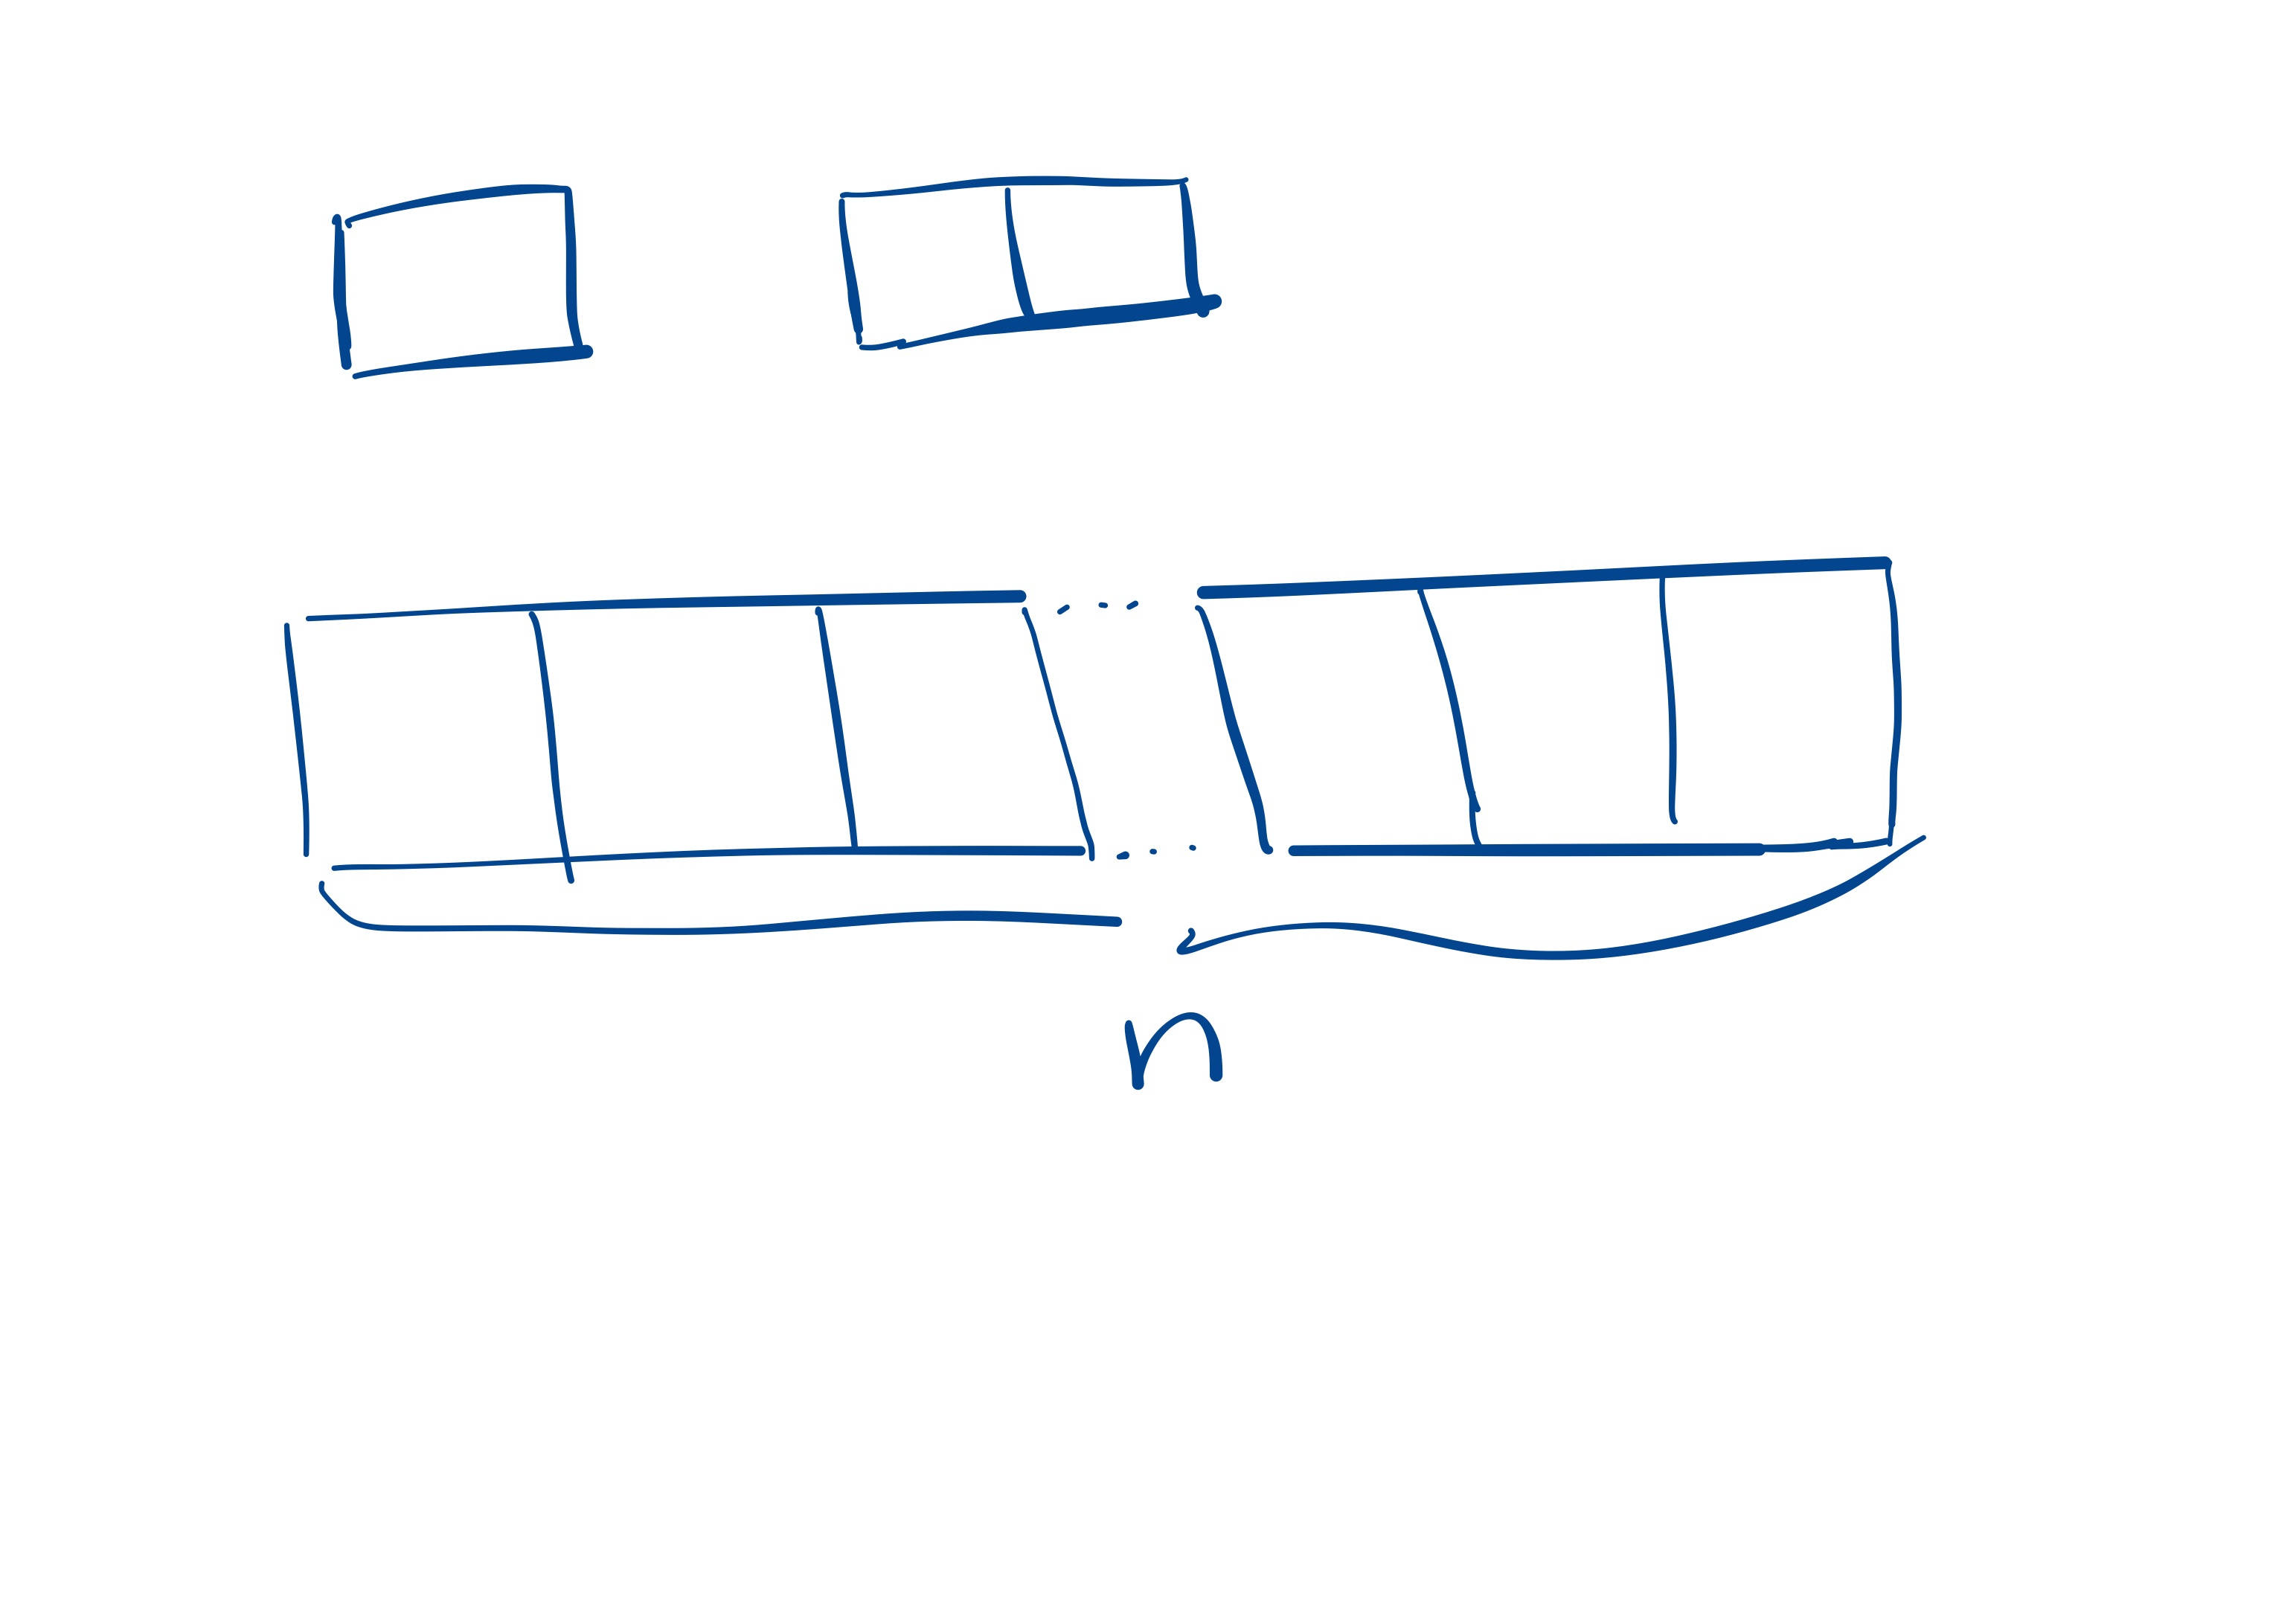
\includegraphics[width=0.8\textwidth]{images/line}
	\caption{Полоска длины n}
\end{figure}
\\Вопрос: сколькими различных способами это можно сделать. Обозначим количество способов $f_n$ и докажем комбинаторно, что оно
будет удовлетворять следующей реккуренте:
\[
	f_n = f_{n - 1} + f_{n - 2}
.\]
В левой части уравнения находится количество способов разделить прямоугольниик $1 \times n$,
указанными способами. \\
Теперь рассмотрим несколько вариантов:
\begin{enumerate}
	\item Отрежем от нашей полоски доминошку, тогда ее длина станет равна $n - 2$.
		Тогда число способов разделить оставшуюся часть полоски будет равно $f_{n - 2}$.
	\item Отрежем квадрат от нашей полоски. По тем же соображение, количество
		способов поделить оставшуюся полоску будет равно $f_{n - 1}$.
\end{enumerate}
Таким образом мы исчерпаем всевозможные способы разделить полоску на квадраты и доминошки. \\
Заметим, что при $n = 1$: $f_1 = 1$, $n = 2$: $f_2 = 2$ и 
условимся, что для $n = 0$: $f_0 = 1$,
так как полоску нулевой длины можно разделить лишь одним способом – "никак". \\
Таким образом, мы доказали представленное выше реккурентное соотношение для известных
чисел Фибоначчи.
\[
	F(s) = \sum_{n=0}^{\infty} f_ns^n = 1 + s + 2s^2 + 3s^3 + 5s^4 + \ldots
\]
Выведем замкнутую форму производящей функции:
\begin{align*}
	F(s) &= \sum_{n=0}^{\infty} f_ns^n = 1 + s + \sum_{n=2}^{\infty} f_ns^n =
	1 + s + \sum_{n=2}^{\infty} (f_{n - 1} + f_{n - 2})s^n = \\ 
		 &= 1 + s + s\left(\sum_{n=2}^{\infty} f_{n - 1}s^{n - 1}\right) +
	s^2\left( \sum_{n=2}^{\infty} f_{n - 2}s^{n - 2} \right) = \\
		 &= 
		 1 + s + s\left(-1 + f_0 + \sum_{n=2}^{\infty} f_{n - 1}s^{n - 1}\right) +
		 s^2\left( \sum_{n=2}^{\infty} f_{n - 2}s^{n - 2} \right) = \\
		 &=
		 1 + s + s\left(-1 + F(s)\right) + s^2F(s) = \\
		 &=
		 1 + sF(s) + s^2F(s) \\
	F(s) &= 1 + s + 2s^2 + 3s^3 + 5s^4 + \ldots = \frac{1}{1 - s - s^2}
.\end{align*}
Заметим, что производящие функции удовлетворяют операции дифференцирования:
\[
	\left(\frac{1}{1 - s - s^2}\right)_s' = (1 + s + 2s^2 + \ldots)_s' =
	 1 + 4s + 9s^2 + 20s^3\ldots = \frac{2s+1}{(1 - s - s^2)^2}
.\] 
\end{document}
